%\newpage
%$ $
%\newpage

\renewcommand{\thesubsection}{\textcolor{red}{\Roman{section}.\arabic{subsection}}}
\renewcommand{\thesubsubsection}{\textcolor{red}{\Roman{section}.\arabic{subsection}.\alph{subsubsection}}}

\setcounter{section}{0}
\sndEnTeteCoursUn

\begin{center}
\begin{mdframed}[style=titr, leftmargin=60pt, rightmargin=60pt, innertopmargin=7pt, innerbottommargin=7pt, innerrightmargin=8pt, innerleftmargin=8pt]

\begin{center}
\large{\textbf{Chapitre 1: Corps purs et mélanges au quotidien}}
\end{center}

\end{mdframed}
\end{center}
Ce chapitre permet de faire une description de la matière à l'échelle macroscopique (c'est-à-dire à notre échelle). Posons-nous les questions suivantes : Qu'est-ce qu'une espèce chimique ? Comment faire pour en identifier une en laboratoire ? Comment reconnaître un mélange d'une espèce chimique unique ?
%
\begin{tcolorbox}[colback=blue!5!white,colframe=blue!75!black,title=Mots clés du chapitre :]
Corps purs, mélange homogène/hétérogène, masse volumique, températures de changement d'état, solubilité.
\end{tcolorbox}

%

\section{Définitions}

\subsection{Espèces chimiques}

La matière est constituée d'\textcolor{red}{entités chimiques} : les atomes, les molécules, les ions. \`{A} partir de ces entités, on peut définir une \textcolor{red}{espèce chimique} :
\begin{tcolorbox}[colback=green!5!white,colframe=green!75!black,title=\textbf{Espèce chimique}, ]
Elle est composée d'un ensemble d'entités chimiques identiques. Une espèce chimique est caractérisée par :
\begin{itemize}
    \item sa formule chimique : par exemple \chemform{H_2O} pour l'eau,
    \item son aspect : couleur, texture, forme, ...
    \item ses propriétés physiques : température d'ébullition, masse volumique, indice de réfraction, ...
    \item ses propriétés chimiques : réactivité avec d'autres espèces chimiques, ... 
\end{itemize}

\end{tcolorbox}

\begin{mdframed}[style=autreexo]
\textbf{\bsc{Exercice de cours 1} - Espèces chimiques}\\
Donner le type (\textit{atomique}, \textit{moléculaire} ou \textit{ionique}) des espèces chimiques suivantes : hélium (He), eau (H\textsubscript{2}O), chlorure de sodium (Na$^{+}$, Cl$^{-}$).
\end{mdframed}
\textit{Réponse :} He : atomique, H\textsubscript{2}O : moléculaire, (Na$^{+}$, Cl$^{-}$) : ionique.

On distingue alors les \textcolor{red}{corps purs} et les \textcolor{red}{mélanges}.

\subsection{Les corps purs}
\begin{tcolorbox}[colback=green!5!white,colframe=green!75!black,title=\textbf{Corps purs}]
Un corps pur est constitué d'une unique espèce chimique.
\end{tcolorbox}

Les corps purs peuvent être :

\begin{itemize}
    \item \textcolor{red}{simples} : ils sont constitués d'un seul type d'atome. Exemples : le dihydrogène \chemform{H_2}, le charbon \chemform{C}, l'argent \chemform{Ag}.
    \item \textcolor{red}{composés} : ils sont constitués de plusieurs atomes dans des proportions bien définies. Exemples : l'eau \chemform{H_2O}, l'éthanol \chemform{C_2H_6O}, le chlorure de sodium \chemform{(Na^+;Cl^-)}.
\end{itemize}

%%%%%%%%



%
\subsection{Le cas des mélanges}
\begin{tcolorbox}[colback=green!5!white,colframe=green!75!black,title=\textbf{Mélange}]
Un mélange est constitué de plusieurs espèces chimiques différentes.
\end{tcolorbox}
Les mélanges peuvent être :
\begin{itemize}
    \item \textcolor{red}{homogènes} : ils sont constitués d'une seule phase (solide, liquide ou vapeur) indiscernable à l'\oe il nu. Lorsque deux liquides se mélangent l'un avec l'autre, on dit qu'ils sont \textcolor{red}{miscibles}.
    \item \textcolor{red}{hétérogènes} : ils sont constitués de plusieurs phases discernables à l'\oe il nu.
\end{itemize}

\begin{mdframed}[style=autreexo]
\textbf{\bsc{Exercice de cours 2} - Corps purs et mélanges}\\
Pour chaque substance suivante, dire s’il s’agit d’un corps pur simple/complexe ou d’un mélange homogène/hétérogène.
\end{mdframed}
\begin{table*}
    \centering
    \begin{tabular}{|C{0.15}|C{0.15}|c|c|C{0.15}|}
    \hline
    Description & Bécher d'huile et d'eau & Bécher d'huile & Bécher d'eau pure & Bécher d'azote liquide \\
    \hline
    Photographie & 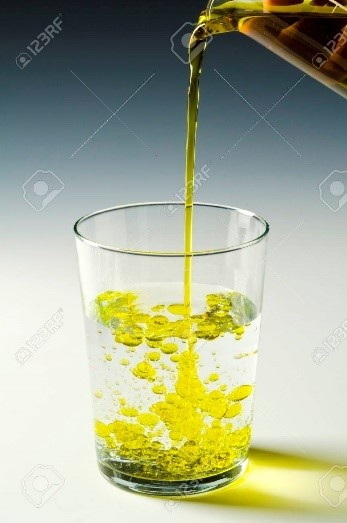
\includegraphics[scale=0.6]{Images/Chapitre_1/Becher_huile_eau.jpg} & 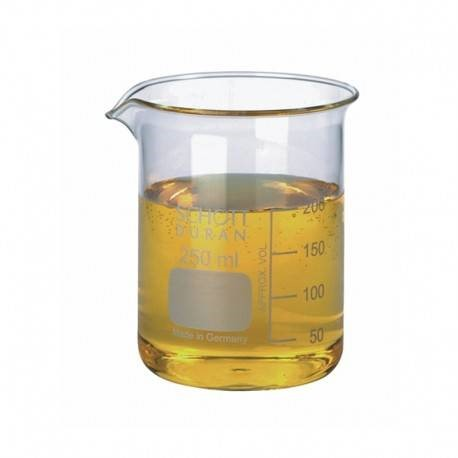
\includegraphics[scale=0.3]{Images/Chapitre_1/Becher_huile.jpg} & 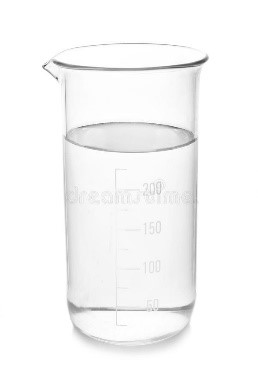
\includegraphics[scale=0.7]{Images/Chapitre_1/Becher_eau.jpg} & 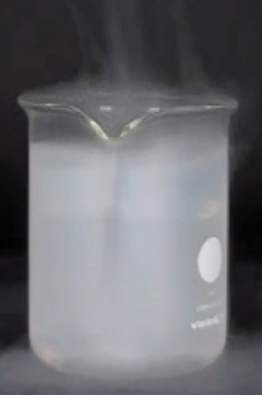
\includegraphics[scale=0.3]{Images/Chapitre_1/Becher_azote.png} \\
    \hline
    Type de corps &  &  &  & \\
    \hline
    Qualificatif du corps & & & &  \\
    \hline
   \end{tabular}
\end{table*}

\section{Identification d'espèces chimiques}
Comment reconnaitre expérimentalement une espèce chimique par rapport à une autre ? On présente dans cette partie quelques éléments qui vont nous permettre de répondre à cette question.

\subsection{Tests chimiques}
\begin{tcolorbox}[colback=red!5!white,colframe=red!75!black,title=\textbf{Tests chimiques à connaître : }]
%\begin{table}
    %\centering
   \begin{tabular}{|C{0.31}|C{0.3}|C{0.31}|}
   \hline
    \cellcolor{blue!25} Espèce chimique à tester & \cellcolor{blue!25} Test & \cellcolor{blue!25} Résultat du test positif \\
    \hline
    Eau (\chemform{H_2O}) & Sulfate de cuivre anhydre (solide blanc)  & Apparition d'un précipité bleu \\
    \hline
    Dioxygène (\chemform{O_2}) & Bûche incandescente & La bûche s'enflamme, incandescence ravivée \\
    \hline
    Dihydrogène (\chemform{H_2}) & Allumette enflammée  &  Détonation \\
    \hline 
    Dioxyde de carbone (\chemform{CO_2}) & Eaux de chaux & Eau de chaux troublée, un précipité blanc appararaît \\
    \hline
    \end{tabular}
%\end{table}
\end{tcolorbox} 

\subsection{Propriétés physiques}
\subsubsection{La masse volumique}
\begin{tcolorbox}[colback=green!5!white,colframe=green!75!black,title=\textbf{Rappel : masse volumique et densité }]
La masse volumique d'une espèce chimique est :
\begin{equation*}
    \rho = \frac{m}{V}
\end{equation*}
avec m la masse de l'espèce et V son volume. Elle s'exprime en g.cm$^{-3}$.\\
La densité $d$ d'une espèce chimique est le rapport entre la masse volumique de cette substance et la masse volumique de l'eau liquide valant $\rho_{eau}=1$~g.cm$^{-3}$ :
\begin{equation*}
    d = \frac{\rho_{espece}}{\rho_{eau}}
\end{equation*}
\importantbox{$d$ s'exprime sans unité puisqu'il s'agit d'un rapport entre deux grandeurs physique de même nature.}
\end{tcolorbox}

\begin{tcolorbox}[colback=red!5!white,colframe=red!75!black,title=\textbf{Masse volumique de l'eau: }]
\begin{center}
    $\rho_{eau} = $1000~kg.m$^{-3}$ ou 1~g.cm$^{-3}$. 
\end{center}
\end{tcolorbox}

\begin{tabular}{|c|C{0.06}|C{0.06}|C{0.06}|C{0.1}|C{0.15}|C{0.1}|C{0.1}|}
   \hline
     & Vide & Air & Eau & Glace & Cyclohexane & Bronze & Or \\
    \hline
    $\rho$ (en g.cm$^{-3}$) & 0 & 0,001 & 1,0 & 0,92 & 0,79 & 7,9 & 19  \\
    \hline
    d & 0 & 0,001 & 1,0 & 0,92 & 0,79 & 7,9 & 19 \\
    \hline
    \end{tabular}
\begin{mdframed}[style=autreexo]
\textbf{\bsc{Exercice de cours 3} - Masse volumique du cyclohexane}\\
\textbf{1)} Calculer la masse volumique du cyclohexane sachant qu'un volume de 15~mL a une masse de 11,8~g.\newline \textbf{2)} Le cyclohexane est-il plus dense que l'eau ? \end{mdframed}
\textit{Réponse :} \\
\textbf{1)}. On calcule la masse volumique du cyclohexane à l'aide de la formule du cours : $\rho=\frac{m}{V} = \frac{11,8}{15}=0,79$~g.mL$^{-1}=0,79$ g.cm$^{-3}$.\\
\textbf{2)}. On déduit la densité à l'aide de la formule du cours et de la question 1) : $d=\frac{\rho_{cyclohexane}}{\rho_{eau}}=\frac{0,79}{1,0}=0,79$. Comme $d<1$, le cyclohexane est moins dense que l'eau. 
\newpage

\subsubsection{Les températures de changement d'état}
\begin{figure}[!htb]
    \centering
    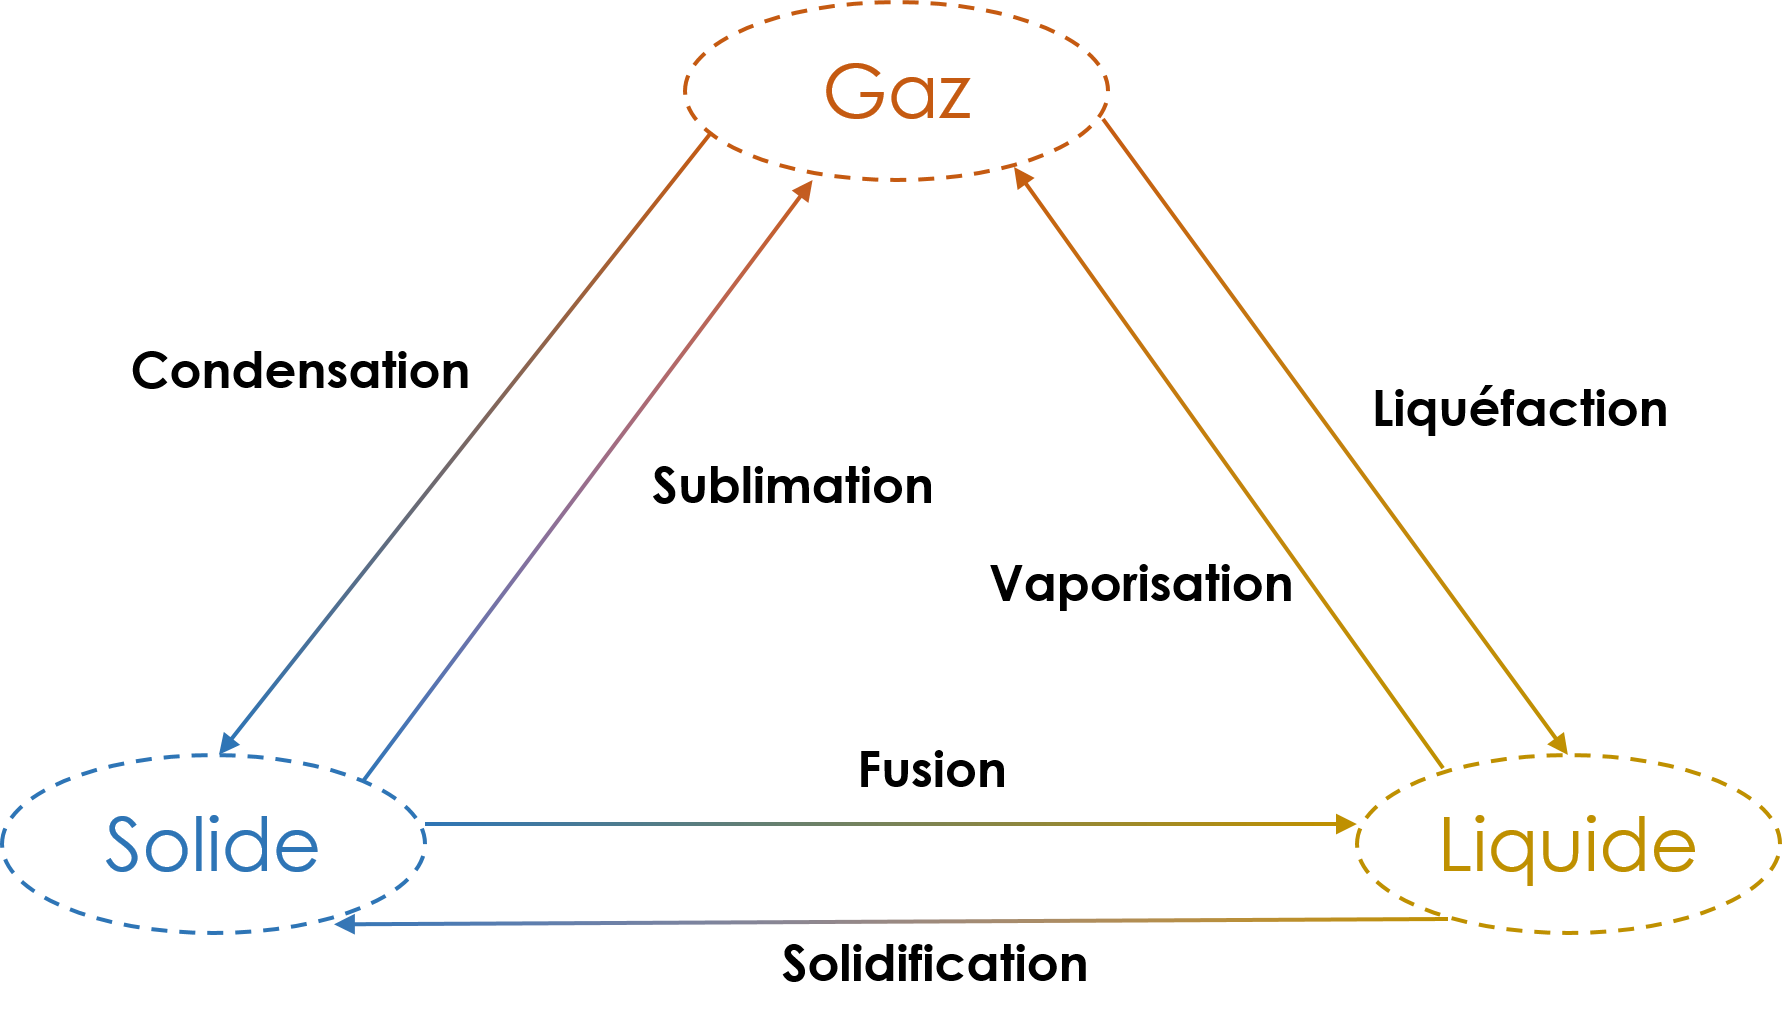
\includegraphics[scale=0.5]{Images/Chapitre_1/Changement_etat_complet.png}
    \caption{Les changements d'états de la matière}
    \label{fig:enter-label}
\end{figure}
Tout changement d'état \underline{d'un corps pur} s'effectue à une température donnée. Il y a deux définitions importantes à connaître :
\begin{itemize}
    \item On appelle \textcolor{red}{température de fusion}, notée $\theta_f$, d'une espèce chimique la température \textbf{à partir de laquelle la phase solide de cette espèce commence à fondre},
    \item On appelle \textcolor{red}{température d'ébullition}, notée $\theta_{eb}$, d'une espèce chimique la température \textbf{à partir de laquelle la phase liquide de cette espèce commence à s'évaporer.} 
\end{itemize}
On verra en TP qu'on peut mesurer une température de fusion à l'aide d'un \textcolor{red}{banc Kofler}.

\begin{minipage}{0.6\textwidth}
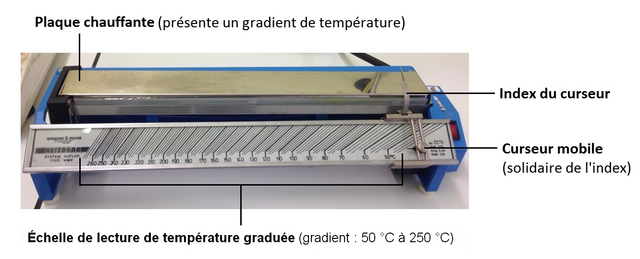
\includegraphics[width=1\textwidth]{Images/Chapitre_1/Banc_Kofler.png} 
  \end{minipage}
\begin{minipage}{0.4\textwidth}
\underline{\textbf{Exemple à connaitre}} :\newline \`{A} une pression de 1~bar, $\theta_{f}(eau)=0\degreCelsius$ et $\theta_{eb}(eau)=100\degreCelsius$
  \end{minipage}



\newpage

\begin{mdframed}[style=autreexo]
\textbf{\bsc{Exercice de cours 4} - Quel état ?}\\
Dans quel état se trouve l'acide citrique à 0~$\degreCelsius$, à température ambiante (20~$\degreCelsius$) et à 100~$\degreCelsius$.\\
\textit{Données :} $\theta_f=153$~$\degreCelsius$ et $\theta_{eb}=310$~$\degreCelsius$
\end{mdframed}
\textit{Réponse :} Les trois températures 0~$\degreCelsius$, 20~$\degreCelsius$ et 100~$\degreCelsius$ sont inférieures à la température de fusion $\theta_f=153$~$\degreCelsius$ de l'acide citrique. Ce dernier est donc solide à ces températures.

\subsection{Chromatograhie sur Couche Mince (CCM)}

\begin{tcolorbox}[colback=green!5!white,colframe=green!75!black,title=\textbf{CCM }]
Une chromatographie sur couche mince est une méthode expérimentale permettant de \textbf{séparer} et \textbf{d'identifier} des éléments chimiques différentes d'un mélange homogène.
\end{tcolorbox}
Elle repose sur la différence d'affinité des espèces chimiques étudiées pour deux phases :
\begin{itemize}
    \item \textbf{la phase fixe} : la plaque chromatographique composée la plupart du temps de silice,
    \item \textbf{une phase mobile} : l'éluant qui va entraîner les espèces à se séparer le long de la phase fixe.
\end{itemize}

\begin{minipage}[c]{0.4\textwidth}
    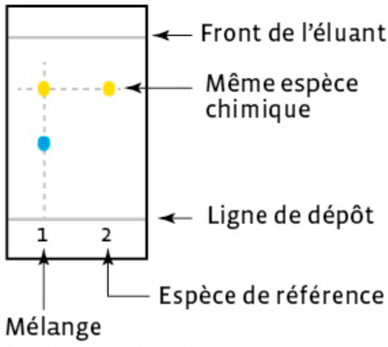
\includegraphics{Images/Chapitre_1/CCM.png}
\end{minipage}
\begin{minipage}[c]{0.6\textwidth}
    \textbf{Lecture d'un chromatogramme} :
    \begin{itemize}
        \item \underline{Lecture horizontale :} deux tâches situées à la même hauteur correspondent à la même espèce chimique. Ce sont les tâchs jaunes sur la figures de gauche.
        \item  \underline{Lecture verticale :} si un dépôt donne plusieurs tâches (comme c'est le cas sur la figure de gauche), alors il est constitué de plusieurs espèces chimiques : c’est un mélange.
    \end{itemize}
\end{minipage}

\section{Composition d'un mélange}
On vient de voir dans la partie précédente comment identifier une ou plusieurs espèces chimiques en fonction de ses propriétés physico-chimiques. Mais comment donne-t'on la composition d'un mélange ? On introduit ici la proportion volumique et massique d'une espèce dans un mélange.

\subsection{Proportion volumique et massique}

\begin{tcolorbox}[colback=green!5!white,colframe=green!75!black,title=\textbf{Proportion volumique}]
La proportion en volume (ou volumique) d'une espèce dans un mélange est le quotient du volume $V_{E}$ qu'occupe cette espèce par le volume total $V_{tot}$ du mélange :
\begin{equation*}
    \frac{V_E}{V_{tot}}
\end{equation*}
avec $V_{E}$ et $V_{tot}$ exprimées dans la même unité (L ou m$^3$ par exemple)
\end{tcolorbox}

\begin{tcolorbox}[colback=green!5!white,colframe=green!75!black,title=\textbf{Proportion massique}]
La proportion en masse (ou massique) d'une espèce dans un mélange est le quotient de la masse $m_{E}$ de cette espèce dans le mélange par la masse totale $m_{tot}$ du mélange :
\begin{equation*}
    \frac{m_E}{m_{tot}}
\end{equation*}
avec $m_{E}$ et $m_{tot}$ exprimées dans la même unité (g ou kg par exemple).
\end{tcolorbox}

Ces proportions peuvent être exprimées en \% et sont sans unités puisqu'il s'agit d'un rapport en deux grandeurs sans unités.

\subsection{Exemple à connaître : la composition de l'air}
L'air est un mélange de gaz indispensable à la vie sur Terre. Quand il est sec, c'est-à-dire qu'il ne contient pas de vapeur d'eau, voici sa composition :
\begin{figure}[!hbt]
    \centering
    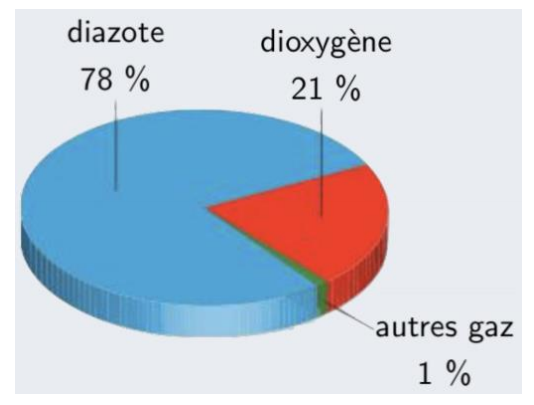
\includegraphics[scale=0.5]{Images/Chapitre_1/Composition_air.png}
    \caption{Diagramme de la composition de l'air}
    \label{fig:compo_air}
\end{figure}

\begin{mdframed}[style=autreexo]
\textbf{\bsc{Exercice de cours 5} - Proportion}\\
A partir du diagramme présenté sur la figure, donnez le volume occupé par le diazote et le dioxygène pour un volume d'air total de $100$~L.
\end{mdframed}
\textit{Réponse :} Diazote : $V_{N_2}=78\%*100=78$~L. Dioxygène : $V_{O_2}=21\%*100=21$~L.

